\chapter{Discussion}\label{ch7:discuss}

Risk acts as a significant barrier to the adoption of geothermal energy as part of a larger energy portfolio for commercial oil \& gas companies. Here, the word “risk” refers to the uncertainty in future conditions that, with some probability of occurrence, could result in an undesirable or unacceptable level of loss.  Companies considering investments in geothermal want to minimize risk exposure, so strategies to mitigate this risk will naturally act as enablers for investment in geothermal during the on-going energy transition.

Maturing a geothermal asset from initial concept through site decommissioning represents a complex project lifecycle spanning up to several decades in length. Figure \ref{fig:geothermal_field_lifecycle} illustrates the decomposition of a geothermal field lifecycle into a level 1 process flow that mimics that of a typical hydrocarbon field. The level 2 decomposition describes a work breakdown structure, each step with its own inherent risks. Here, the primary play risk elements for geothermal introduced in Section \ref{ch2:sysfund} have been reframed as four components: heat, permeability, fluids, and seal. Each appear in both the Exploration and Appraisal phases of the project. 

\begin{figure}[!htp]
\centering
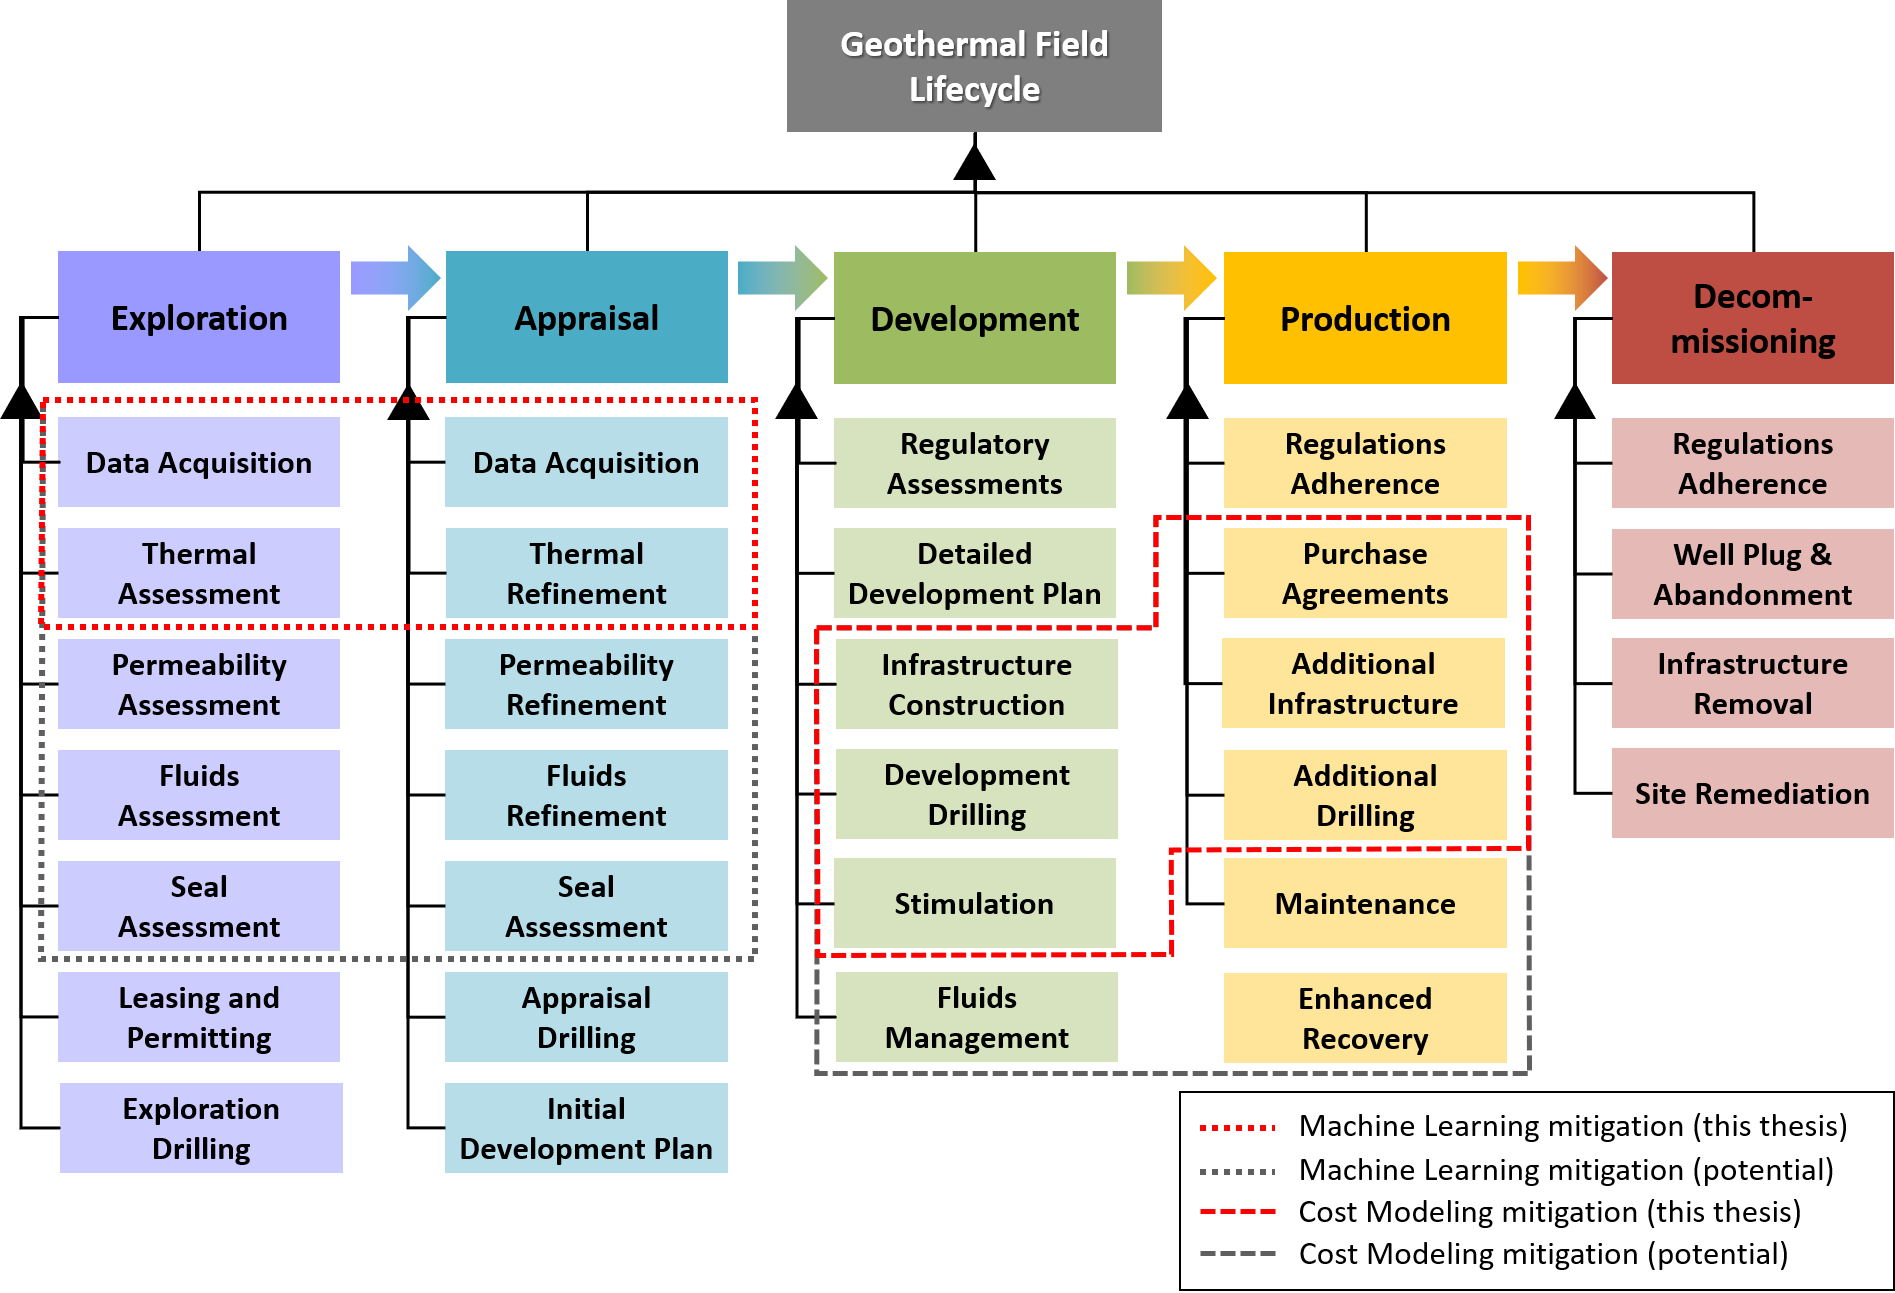
\includegraphics[width=\textwidth]{templates/images/Figure-SystemDecomposition.png}
\caption[Geothermal field lifecycle]{Caption}
\label{fig:geothermal_field_lifecycle}
\end{figure}

The red dotted outline in Figure \ref{fig:geothermal_field_lifecycle} illustrates activities in the Exploration and Appraisal stages where machine learning methods described in Chapters 3 and 5 can reduce the overall risk profile. Geothermal exploration commonly focuses on areas where data and known resources are already present. Reviewing available data to identify feature relationships suggestive of favorable locations is an early pre-screening activity for mitigating the risk of costly exploration failures \citep{doughty_geovision_2018}. ML algorithms described in Chapter 5 provide data-driven methods for uncovering these complex feature relationships and generating resource favorability maps rapidly and at low cost. Furthermore, feature importances derived directly from recursive feature elimination (Section \ref{ch5:logreg_rfe}), impurity measures like Gini index or entropy (Section \ref{ch5:impurity}), or Shapley analysis (Section \ref{ch5:xgb_shapley}) directly rank different data sources by their value for predictive modeling. These measures could also be used to guide exploration and appraisal spending on additional data or acquisition efforts. For example, recognizing that silica geothermometer temperatures, heat flow measurements, crustal thickness, and density of volcanic dikes and springs all highly influence the XGBoost classification model based on Shapley values (see Section \ref{ch5:xgb_shapley}), an exploration team could focus time and budget dollars on 1) field surveys for silica concentration sampling, 2) field or remote-sensing mapping of springs and dikes, and 3) seismic acquisition for improved crustal thickness estimates where those estimates are least well-constrained. 